\chapter{Verloop van het Onderzoek}
\label{onderzoek}

\section{Is het mogelijk om digitaal te gaan?}
\label{onderzoeksvraag1}

Deze sectie gaat na welke methode van geluidsverwerking het best toegepast wordt bij het schrijven van verwerkingsprogramma's. Uit het interview van \textcite{thomashouthave} bleek dat hij het meest intuïtief overweg gaat met subtractive synthesis. In sectie \ref{methode:subtractive} wordt besproken hoe deze methode werkt. \textcite{thomashouthave} meldt in zijn interview dat equalizers en compressors een uitwerking van subtractive synthesis zijn. De andere interviewees vermeldden ook dat zij extensief gebruik maken van equalizers en compressors. Het artikel van \textcite{filtervseq} biedt hier meer inzicht op.

\subsection{Geluidsfilters}

Filters maken prominent deel uit van de subtractive methode zoals in sectie \ref{methode:subtractive} beschreven staat. \textcite{filtervseq} spreekt over de gelijkenissen en verschillen tussen audio equalization en filtering. Waar equalizers bepaalde delen van het frequentiespectrum van een geluid versterken, knippen filters ze af. Beide kunnen gebaseerd worden op een Fast Fourier Transformatie (FFT)\footnote{\textit{fouriereq} leggen in hun onderzoek een toepassing van equalizers uit voor gehoorapparaten. Het idee is om een equalizer in gehoorapparaten te implementeren die bepaalde frequenties verluidt. Die frequenties worden gekozen op basis van het audiogram van de patient. Een audiogram geeft weer vanaf welke amplitude een patient een zekere frequentie kan horen. Zo worden enkel de moeilijk te horen frequenties versterkt. Dit wordt verwezenlijkt door middel van FFT.}. Het enige verschil tussen de twee is de amplitudinale impact. Een equalizer versterkt het geluid rond een zekere frequentie terwijl een filter het verzacht.

Niet alleen biedt FFT meerdere toepassingen in subtractive synthesis. Het biedt ook een tijdscomplexiteit van $\mathcal{O}(n\log{}n)$ die meer acceptabel is dan die van de Discrete Fourier Transformatie (DFT) van $\mathcal{O}(n^2)$.\autocite{ffttime} Het is niet optimaal, daarom worden er reeds tal van onderzoeken gevoerd om de tijdscomplexiteit te verminderen in software aan de hand van multicore computing. \autocite{robbievincke}

De bespreking van FFT is ter illustratie dat equalizers gebaseerd zijn op subtractive synthesis. Er zijn tal van toepassingen van FFT in geluidsfilters maar in software is het typisch niet de verkozen transformatie. Dit omdat het beter gebruikt wordt voor de spectroscopie van frequenties van continue signalen. De sound synthesis libraries besproken in sectie \ref{sec:libraries} maken hier gebruik van de bilineaire tranformatie \autocite{jsynbiquad} omdat die beter toepasbaar is op de real-time verwerking van discrete signalen\footnote{\textcite{rbj} bespreekt in zijn artikel zijn algoritme voor de bilineaire transformatie.}. \textcite{rbj} toont in zijn artikel hoe verschillende filter types geïmplementeerd kunnen worden aan hand van deze transformatie.

\subsection{Harmonisch rijke golven}

Op eerste zicht lijkt het per definitie onmogelijk voor een computer om harmonisch rijke golven te genereren. \textcite{fourier} vertellen het verhaal van Joseph Fourier. In de 19\textsuperscript{de} eeuw stelde hij de hypothese dat alle periodieke functies beschreven kunnen worden als een oneindige som van sinusfuncties - vandaar de benoeming \textit{harmonisch rijk}. Twee jaar voor zijn dood, in 1828, werd dit bewezen door Johann Dirichlet, een wiskundige met wie Fourier correspondentie voerde. Het zijn deze periodieke golven waar subtractive synthesis zich op baseert. \autocite{fourier}

\begin{figure}
\centering
\begin{verbatim}
Function<Double, Double> square = (x) -> (x % p) < (p / 2) ? -1.0 : 1.0;
\end{verbatim}
\caption{Java blokgolf generatie functie}
\label{squarefunction}
\end{figure}

Het is computationeel onmogelijk om een oneindige som van sinusfuncties te genereren.  Maar in se is dat ook niet nodig. Evenals analoge synthesizers genereren de libraries uit sectie \ref{sec:libraries} hun harmonisch rijke golven door middel van logica in plaats van goniometrie. Zo kan de generatie van een harmonisch rijke functie vaak ondergebracht worden in één bewerking. Een voorbeeld in Java: functie \ref{squarefunction} genereert een blokgolf met periode \verb+p+ gegeven een abcis \verb+x+.

De resultaten van deze discrete functies zijn slechts een benadering van die van de continue Fourier series. \autocite{fourier} De geluidsresolutie van vandaag is hoog genoeg dat dit voor het menselijk gehoor nauwelijks zou mogen verschillen. \autocite{vagabundos}

\section{In het nuttig om digitaal te gaan?}

De interviewees hebben elk laten weten wat zij dachten van een digitalisatie. Deze sectie bespreekt aan de hand van hun antwoorden of er in de markt vraag naar is. Het aantal interviews is te klein om een populatie te representeren. Desondanks spreken de interviewees uit jaren van vakkundige ervaring. Daarom kunnen hun antwoorden toch als representabel geacht worden.

\subsection{Is het mogelijk om digitaal te gaan?}

\begin{quotation}
\textbf{Bart Vincent}: \textit{•}

\textbf{Thomas Houthave}: 

\textbf{Peter Boone}: 

\textbf{Vagabundos}: 
\end{quotation}



\subsection{Wie heeft baat bij een digitalisering?}



\subsection{Zou een digitalisering verwelkomd worden?}



\section{Is het realistisch om digitaal te gaan?}

Voor dit onderzoek zijn er performantiemetingen uitgevoerd op de drie libraries die beschreven staan in sectie \ref{sec:libraries}. In sectie \ref{subsec:vergelijkinglibraries} werd de gelijkenis in architectuur tussen de drie libraries vergeleken. Toch brachten ze verbazingwekkend verschillende testresultaten op. In deze sectie worden de verwerking van de resultaten besproken. 

Om antwoord te kunnen geven op de onderzoeksvraag, zou slechts één van de libraries moeten slagen op deze test. Slagen voor deze test houdt in dat de library bij iedere testcase aanvaardbaar performant draait. Hou er rekening mee dat de tests op een ietwat zwakke testmachine draaiden die besproken is in sectie \ref{subsec:methodologie:testmachine}.

In sectie \ref{subsub:testframework} wordt besproken hoe de testresultaten verkregen zijn. Deze zijn terug te vinden in appendix \ref{ch:testresultaten}. Vervolgens werden er twee smoothing methodes op de testresultaten uitgevoerd zoals besproken in sectie \ref{sec:methodologie:verwerking}. In appendix \ref{ch:smoothing} staan de resultaten van beide deze methodes. Hier wordt de verwerking van één testcase besproken: processor verbruik in testcase 4 van JSyn.

\begin{figure}
    		\centering
    		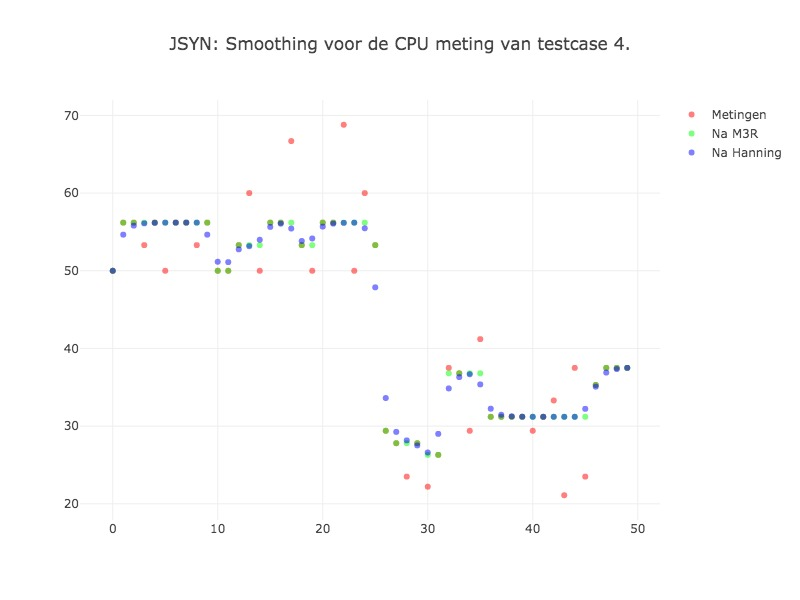
\includegraphics[width=0.75\linewidth]{medians/jsyn_cpu_4}
    		\caption{Smoothing van CPU testresultaten van testcase 4  voor JSyn}
    		\label{jsyn_cpu_4}
\end{figure}

Figuur \ref{jsyn_cpu_4} toont de smoothing van een testcase. De rode punten zijn de originele metingen van de testcase. Als eerste wordt een dubbele \textit{median three smoothing} (M3R) toegepast; besproken in \ref{sec:methodologie:verwerking}. Dit resulteert in de groene set. M3R verwijdert plotse extrema uit het verloop van de meting. Vervolgens is op de resulterende dataset de Hanning vensterfunctie uitgevoerd. Dit leverde de blauwe puntenset op. Hanning maakt dat langere periodes van plotse extrema mooi geëgaliseerd worden.

De mediaan van de dataset die resulteerde uit de Hannign functie werd genomen als resultaat van de meting. In dit voorbeeld is de mediaan \verb+48.93%+. Hieruit kunnen we concluderen dat JSyn doorgaans \verb+48.93%+ van de processorkracht gebruikt op de besproken testmachine.

\begin{table}[]
\centering
\begin{tabular}{l|c|l|l}
\textbf{Library} & \textbf{Case} & \textbf{Mediaan \%CPU} & \textbf{Mediaan \%Mem} \\ \hline
\multicolumn{1}{c}{\multirow{6}{*}{\textbf{Beads}}} & 1             & 6.23      & 0.70     \\
\multicolumn{1}{c}{}                                & 2             & 24.12      & 0.80    \\
\multicolumn{1}{c}{}                                & 3             & 68.80      & 0.80         \\
\multicolumn{1}{c}{}                                & 4             & 87.50     & 1.10           \\
\multicolumn{1}{c}{}                                & 5             & 92.59    & 1.50                  \\
\multicolumn{1}{c}{}                                & 6             & 87.50    & 1.10       \\ \hline
\multirow{6}{*}{\textbf{JASS}}                      & 1             & 93.80     & 0.90          \\
                                                    & 2             & 93.80   & 1.00                    \\
                                                    & 3             & 100.00        & 1.10    \\
                                                    & 4             & 100.00     & 1.20         \\
                                                    & 5             & 100.00                  & 1.30           \\
                                                    & 6             & 100.00      & 1.90           \\ \hline
\multirow{6}{*}{\textbf{JSyn}}                      & 1             & 11.42    & 2.10           \\
                                                    & 2             & 19.05   & 2.30   \\
                                                    & 3             & 33.30     & 2.30         \\
                                                    & 4             & 48.93    & 2.30          \\
                                                    & 5             & 68.81    & 2.30         \\
                                                    & 6             & 56.20    & 2.2930       \\ \hline
\end{tabular}
\caption{Medianen van de verwerkte testresultaten per library per testcase.}
\label{medians}
\end{table}

Alle berekende medianen staan in tabel \ref{medians}. Opvallend is dat JASS al snel aan 100\% processor vermogen zit. Waarom wordt duidelijk na het lezen van de broncode. Voor het opstellen van de testcases van JASS is de \verb+Sine+-klasse gebruikt want het is de enige oscillator aanwezig in de library. \textcite{jasscode} vermeldt in de broncode van de klasse dat dit een \textit{``highly inefficient implementation''} is.



